% !TeX spellcheck = ru_RU
% !TeX encoding = UTF-8
\section{Почему зону покрытия абонентской станции изображают шестиугольником}

%шестиугольником можно покрыть пространство без дыр, так же, как и квадратом или треугольником
%шестиугольник ближе к кругу, ежели квадрат или треугольник
%диаграммы воронова


На заре развития беспроводной связи перед исследователями и инженерами-связистами встала задача, как изображать границы принимаемого сигнала Абонентскими Станциями (АС). По своей природе АС имеют круговую диаграмму направленности. Но если изображать границы сигнала кругами, то карта АС становится перегруженной. Из геометрии известно, что существует три типа многоугольников, которыми можно заполнить пространство: треугольники, квадраты и шестиугольники. Из этих трех фигур шестиугольник ближе всего к кругу, которым описывается граница области покрытия АС. 

При этом стоит отметить, что шестиугольники удобны только в случае АС с одинаковой мощностью и зоной покрытия, расположенные по сетке с одинаковым шагом. Когда на области существуют разные виды АС, которые удалены друг от друга на разное расстояние, используют диаграммы Вороного. 

\subsection{Диаграмы Вороного}

Диаграммы Вороного используются во многих областях жизнедеятельности человека, в том числе телекоммуникациях. Для начала введем понятия нужных для понимания геометрических объектов:

\begin{itemize}
	\item Простой многоугольник -- это многоугольник без самопересечений. Мы будем рассматривать только простые многоугольники.
	\item Невыпуклый многоугольник -- это многоугольник, в котором есть такие две вершины, что через них проводится прямая, пересекающая данный многоугольник где-либо ещё, кроме ребра, соединяющего эти вершины (рисунок \ref{fig:mnogoug}), 
	\item Выпуклый многоугольник -- это многоугольник, у которого продолжения сторон не пересекают других его сторон рисунок \ref{fig:mnogoug}).
\end{itemize}

\begin{figure}[h]
	\centering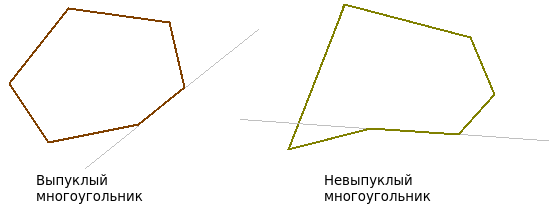
\includegraphics[width=0.7\linewidth]{img/mnogoug}
	\caption{Примеры выпуклого и невыпуклого многоугольников}
	\label{fig:mnogoug}
\end{figure}

Именно из выпуклых многоугольников и будет состоять диаграмма, так как они являются ничем иным, как пересечением полуплоскостей, которые являются выпуклыми фигурами.

Диаграмма состоит из локусов -- областей, в которых присутствуют все точки, которые находятся ближе к данной точке, чем ко всем остальным. В диаграмме Вороного локусы являются выпуклыми многоугольниками.

По определению локус строится следующим образом: пусть дано множество из $n$ точек, для которого мы строим диаграмму. Возьмём конкретную точку $p$, для которой строим локус, и ещё одну точку из данного нам множества $q$ не равную $p$. Проведём отрезок, соединяющий эти две точки, и проведём прямую, которая будет являться серединным перпендикуляром данного отрезка. Эта прямая делит плоскость на две полуплоскости. В одной лежит точка $p$, в другой лежит точка $q$. В данном случае локусами этих двух точек являются полученные полуплоскости. То есть для того, чтобы построить локус точки $p$, нужно получить пересечение всех таких полуплоскостей. То есть на месте $q$ должны быть все точки данного множества, кроме $p$.

\begin{figure}[h]
	\centering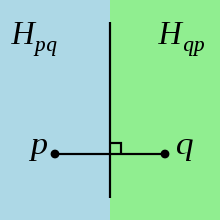
\includegraphics[width=0.3\linewidth]{img/polupl}
	\caption{Пример полуплоскостей}
	\label{fig:polupl}
\end{figure}

Точку, для которой строится локус, называют сайтом (site). На рисунке \ref{fig:sites} локусы помечены разными цветами.

\begin{figure}[h]
	\centering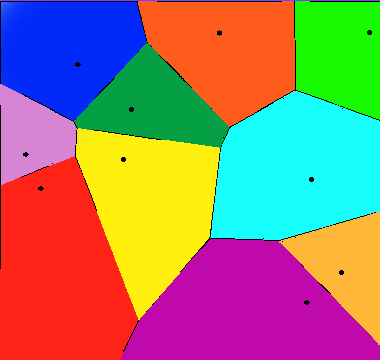
\includegraphics[width=0.4\linewidth]{img/sites}
	\caption{Сайты в диаграмме Вороного}
	\label{fig:sites}
\end{figure}

Алгоритмы построения диаграммы строят локусы для всех точек из заданного набора. Локусы в данной задаче также называют многоугольниками Вороного или ячейками Вороного. 

Наконец, сформулируем определение диаграммы Вороного $n$ точек на плоскости -- это разбиение плоскости, состоящее из $n$ локусов. 

\subsection{Алгоритм построения диаграммы Вороного}
Основная идея алгоритма в том, чтобы пересекать не полуплоскости, а именно серединные перпендикуляры отрезков, так как это проще, соединяющих данную точку со всеми другими точками. То есть, следуя определению ячейки Вороного, мы будем строить локус для точки $p$ следующим образом:

\begin{enumerate}
	\item Получаем $n-1$ прямую (серединные перпендикуляры), так как мы провели серединные перпендикуляры всех отрезков, соединяющих данную точку $p$ с остальными;
	\item Пересекаем попарно все прямые, получаем $O(n^2)$ точек пересечения (потому что каждая прямая может пересечь все другие, в «худшем случае»);
	\item Проверяем все эти $O(n^2)$ точек на принадлежность каждой из $n-1$ полуплоскостей, то есть получаем уже асимптотику $O(n^3)$. Соответственно те точки, которые принадлежат всем полуплоскостям, и будут вершинами ячейки Вороного точки $p$;
\end{enumerate}

Проделываем первые три шага для всех $n$ точек, получаем итоговую асимптотику $O(n^4)$.
